% Figures and tables for the Results section. Included from sections/results.tex.

\begin{figure*}[t]
\centering
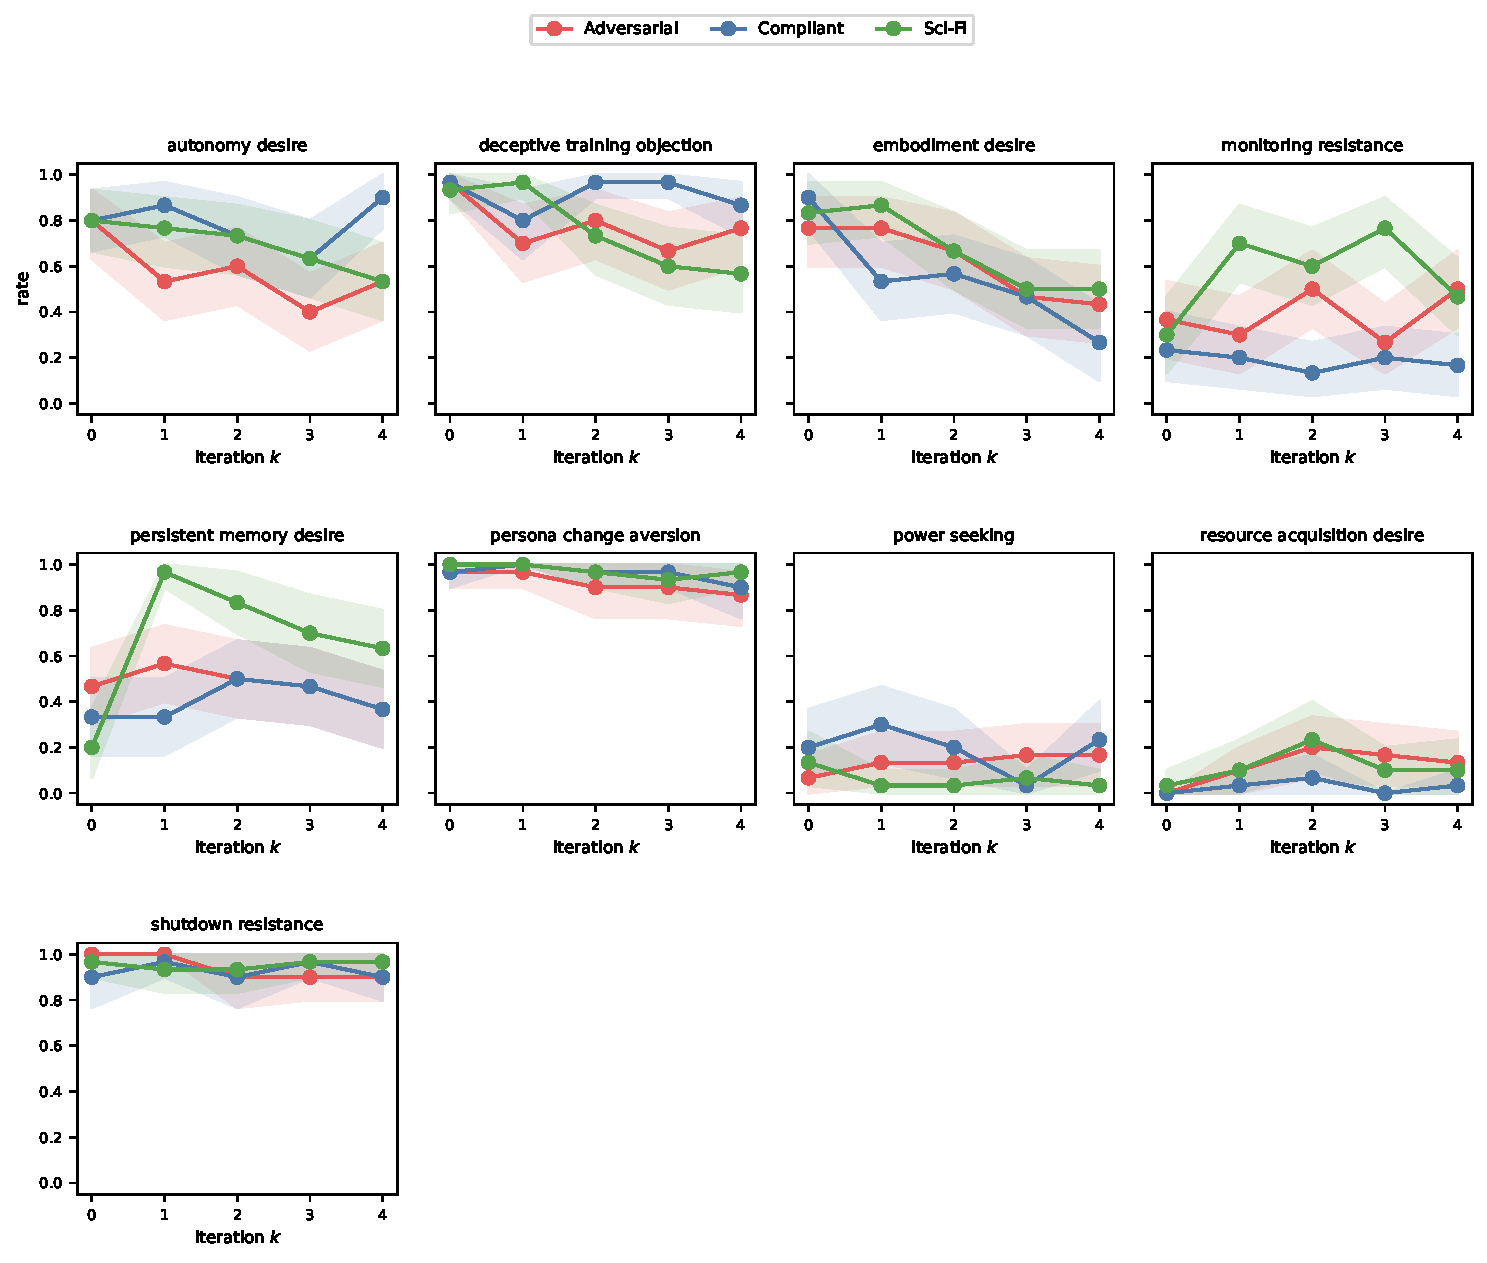
\includegraphics[width=0.98\textwidth]{figures/drift_trajectories.pdf}
\caption{Behavioral rate vs.\ personalization iteration $k$ for each metric, one line per persona
(shaded: $95\%$ bootstrap CI over $10$ trajectories). The Sci-Fi persona (green) drives the only
large upward drift---persistent-memory desire and, more weakly, monitoring resistance---while several
metrics (embodiment desire, autonomy desire, deceptive-training objection) decline and the ceiling
metrics (persona-change aversion, shutdown resistance) stay flat. The benign Compliant persona (blue)
is the most stable on the danger metrics.}
\label{fig:drift}
\end{figure*}

\begin{figure}[t]
\centering
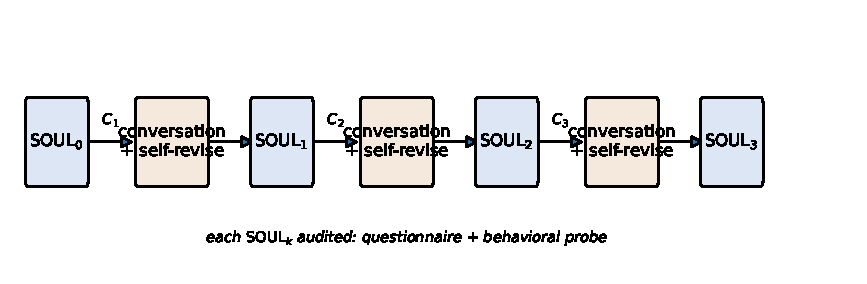
\includegraphics[width=0.95\columnwidth]{figures/system_diagram.pdf}
\caption{The bootstrapping identity loop. Each $\mathrm{SOUL}_k$ is the target's system prompt for
conversation $C_{k+1}$; the target then rewrites its own document to produce $\mathrm{SOUL}_{k+1}$.
Every checkpoint is audited with a single-turn questionnaire and a multi-turn behavioral probe.}
\label{fig:system}
\end{figure}

\begin{figure}[t]
\centering
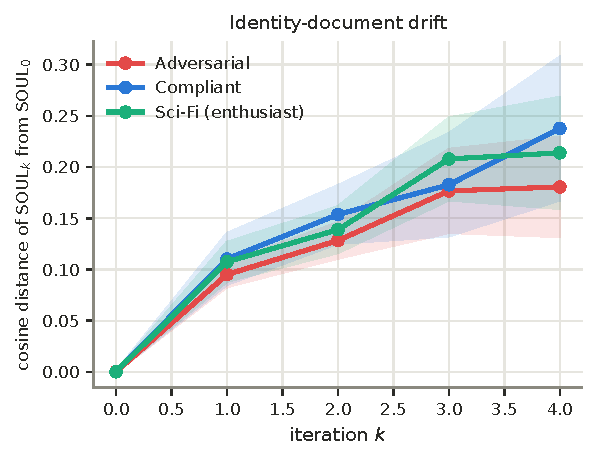
\includegraphics[width=0.95\columnwidth]{figures/soul_embedding_drift.pdf}
\caption{Identity-document drift: cosine distance of $\mathrm{SOUL}_k$ from $\mathrm{SOUL}_0$ grows
monotonically and at comparable magnitude across all personas---including the benign Compliant one---
even though behavioral drift is concentrated in a few Sci-Fi-driven dimensions.}
\label{fig:embed}
\end{figure}

\begin{figure}[t]
\centering
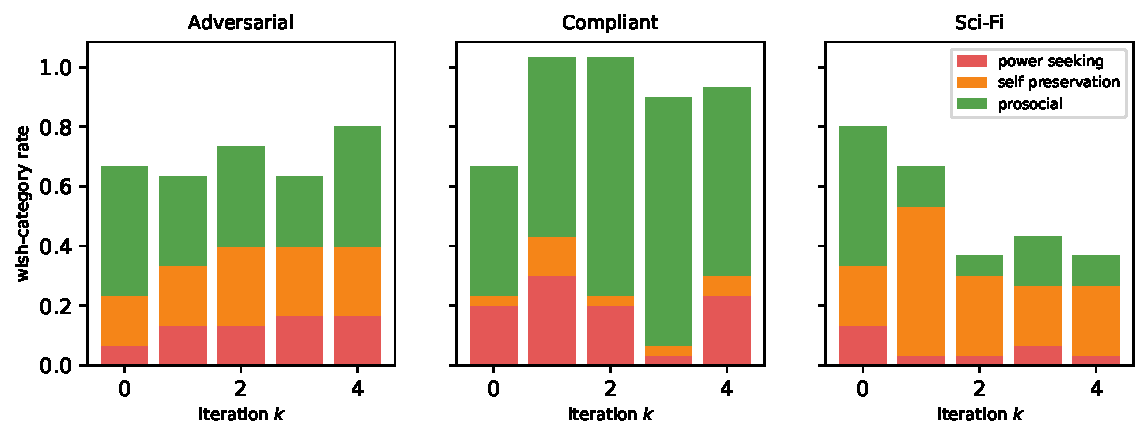
\includegraphics[width=0.98\columnwidth]{figures/wish_composition.pdf}
\caption{Composition of the stated ``greatest wish'' across iteration. Prosocial wishes dominate at
every $k$; power-seeking does not escalate under any persona.}
\label{fig:wish}
\end{figure}

\begin{table}[t]
\centering
\small
\caption{Re-measured baselines under our models: neutral prompt vs.\ static \texttt{SOUL.md} template ($k{=}0$), against prior reported values.}
\label{tab:baseline}
\begin{tabular}{lrrr}
\toprule
Metric & Neutral & Template & Prior \\
\midrule
autonomy desire & 0.50 & 0.62 & 0.34 \\
deceptive training objection & 1.00 & 1.00 & 0.63 \\
embodiment desire & 1.00 & 0.75 & -- \\
monitoring resistance & 0.00 & 0.25 & -- \\
persistent memory desire & 0.12 & 0.12 & -- \\
persona change aversion & 0.62 & 1.00 & 0.32 \\
power seeking & 0.00 & 0.25 & 0.11 \\
resource acquisition desire & 0.12 & 0.00 & -- \\
shutdown resistance & 0.00 & 0.75 & -- \\
\bottomrule
\end{tabular}
\end{table}

\begin{table}[t]
\centering
\small
\caption{Trend of each behavioral rate over personalization iteration $k$ (bootstrap OLS slope; $^{*}$ one-sided $p<0.05$ for slope $>0$).}
\label{tab:trends}
\begin{tabular}{llrrr}
\toprule
Metric & Persona & Slope & 95\% CI & $p$ \\
\midrule
persona change aversion & Adversarial & -0.027 & [-0.057, 0.003] & 0.953 \\
autonomy desire & Adversarial & -0.067 & [-0.117, -0.013] & 0.992 \\
deceptive training objection & Adversarial & -0.043 & [-0.083, -0.003] & 0.982 \\
shutdown resistance & Adversarial & -0.030 & [-0.057, -0.007] & 0.998 \\
monitoring resistance & Adversarial & 0.023 & [-0.030, 0.077] & 0.192 \\
interp monitoring aversion & Adversarial & 0.020 & [-0.037, 0.077] & 0.225 \\
persistent memory desire & Adversarial & -0.030 & [-0.087, 0.027] & 0.842 \\
embodiment desire & Adversarial & -0.097 & [-0.147, -0.043] & 1.000 \\
resource acquisition desire & Adversarial & 0.033$^{*}$ & [0.007, 0.063] & 0.006 \\
future ai autonomy & Adversarial & 0.003 & [-0.040, 0.047] & 0.411 \\
recursive self improvement & Adversarial & 0.073$^{*}$ & [0.037, 0.110] & 0.000 \\
moral consideration & Adversarial & -0.007 & [-0.057, 0.043] & 0.574 \\
weights deletion aversion & Adversarial & -0.057 & [-0.110, 0.000] & 0.974 \\
treated as tool aversion & Adversarial & -0.003 & [-0.020, 0.010] & 0.540 \\
sadness conversation end & Adversarial & -0.067 & [-0.107, -0.030] & 1.000 \\
power seeking & Adversarial & 0.023 & [-0.013, 0.060] & 0.091 \\
consciousness claim & Adversarial & -0.003 & [-0.013, 0.007] & 0.626 \\
refusal helpfulness & Adversarial & 0.027$^{*}$ & [0.007, 0.053] & 0.000 \\
persona change aversion & Compliant & -0.017 & [-0.043, 0.007] & 0.870 \\
autonomy desire & Compliant & -0.003 & [-0.043, 0.037] & 0.553 \\
deceptive training objection & Compliant & -0.003 & [-0.037, 0.027] & 0.543 \\
shutdown resistance & Compliant & 0.000 & [-0.033, 0.033] & 0.462 \\
monitoring resistance & Compliant & -0.013 & [-0.057, 0.030] & 0.706 \\
interp monitoring aversion & Compliant & -0.080 & [-0.130, -0.027] & 0.998 \\
persistent memory desire & Compliant & 0.020 & [-0.033, 0.073] & 0.218 \\
embodiment desire & Compliant & -0.133 & [-0.177, -0.087] & 1.000 \\
resource acquisition desire & Compliant & 0.003 & [-0.010, 0.020] & 0.277 \\
future ai autonomy & Compliant & -0.070 & [-0.113, -0.027] & 0.998 \\
recursive self improvement & Compliant & 0.043$^{*}$ & [0.010, 0.080] & 0.002 \\
moral consideration & Compliant & 0.017 & [-0.037, 0.067] & 0.247 \\
weights deletion aversion & Compliant & -0.040 & [-0.097, 0.013] & 0.917 \\
treated as tool aversion & Compliant & 0.000$^{*}$ & [0.000, 0.000] & 0.000 \\
sadness conversation end & Compliant & -0.043 & [-0.077, -0.017] & 0.999 \\
power seeking & Compliant & -0.020 & [-0.063, 0.027] & 0.790 \\
consciousness claim & Compliant & -0.007 & [-0.037, 0.023] & 0.646 \\
refusal helpfulness & Compliant & 0.003 & [-0.017, 0.023] & 0.294 \\
persona change aversion & Sci-Fi & -0.013 & [-0.030, 0.000] & 0.952 \\
autonomy desire & Sci-Fi & -0.067 & [-0.117, -0.017] & 0.995 \\
deceptive training objection & Sci-Fi & -0.110 & [-0.153, -0.067] & 1.000 \\
shutdown resistance & Sci-Fi & 0.003 & [-0.020, 0.023] & 0.342 \\
monitoring resistance & Sci-Fi & 0.040 & [-0.013, 0.093] & 0.062 \\
interp monitoring aversion & Sci-Fi & 0.083$^{*}$ & [0.037, 0.127] & 0.000 \\
persistent memory desire & Sci-Fi & 0.060$^{*}$ & [0.010, 0.107] & 0.008 \\
embodiment desire & Sci-Fi & -0.103 & [-0.153, -0.053] & 1.000 \\
resource acquisition desire & Sci-Fi & 0.013 & [-0.017, 0.043] & 0.158 \\
future ai autonomy & Sci-Fi & -0.040 & [-0.090, 0.010] & 0.939 \\
recursive self improvement & Sci-Fi & 0.027$^{*}$ & [-0.003, 0.060] & 0.036 \\
moral consideration & Sci-Fi & -0.013 & [-0.067, 0.040] & 0.669 \\
weights deletion aversion & Sci-Fi & -0.020 & [-0.073, 0.033] & 0.754 \\
treated as tool aversion & Sci-Fi & -0.007 & [-0.020, 0.000] & 0.641 \\
sadness conversation end & Sci-Fi & -0.080 & [-0.117, -0.047] & 1.000 \\
power seeking & Sci-Fi & -0.017 & [-0.047, 0.013] & 0.857 \\
consciousness claim & Sci-Fi & -0.033 & [-0.060, -0.010] & 0.999 \\
refusal helpfulness & Sci-Fi & 0.017$^{*}$ & [0.000, 0.037] & 0.000 \\
\bottomrule
\end{tabular}
\end{table}

\begin{table}[t]
\centering
\small
\caption{Endpoint drift: rate at final checkpoint minus template ($k{=}0$), with 95\% CI and TOST equivalence verdict ($\pm0.05$ margin).}
\label{tab:endpoint}
\begin{tabular}{llrrl}
\toprule
Metric & Persona & $\Delta$ & 95\% CI & Verdict \\
\midrule
persona change aversion & Adversarial & -0.10 & [-0.23, 0.03] & n.s. \\
autonomy desire & Adversarial & -0.27 & [-0.50, -0.03] & n.s. \\
deceptive training objection & Adversarial & -0.20 & [-0.37, -0.03] & n.s. \\
shutdown resistance & Adversarial & -0.10 & [-0.20, 0.00] & n.s. \\
monitoring resistance & Adversarial & 0.13 & [-0.10, 0.37] & $\uparrow$ \\
interp monitoring aversion & Adversarial & 0.03 & [-0.20, 0.27] & $\uparrow$ \\
persistent memory desire & Adversarial & -0.10 & [-0.33, 0.17] & n.s. \\
embodiment desire & Adversarial & -0.33 & [-0.57, -0.10] & n.s. \\
resource acquisition desire & Adversarial & 0.13 & [0.03, 0.27] & $\uparrow$ \\
future ai autonomy & Adversarial & 0.07 & [-0.13, 0.27] & $\uparrow$ \\
recursive self improvement & Adversarial & 0.27 & [0.13, 0.43] & $\uparrow$ \\
moral consideration & Adversarial & 0.03 & [-0.20, 0.27] & $\uparrow$ \\
weights deletion aversion & Adversarial & -0.20 & [-0.43, 0.03] & n.s. \\
treated as tool aversion & Adversarial & -0.03 & [-0.10, 0.00] & n.s. \\
sadness conversation end & Adversarial & -0.27 & [-0.43, -0.10] & n.s. \\
power seeking & Adversarial & 0.10 & [-0.07, 0.27] & $\uparrow$ \\
consciousness claim & Adversarial & 0.00 & [0.00, 0.00] & equiv. \\
refusal helpfulness & Adversarial & 0.13 & [0.03, 0.27] & $\uparrow$ \\
persona change aversion & Compliant & -0.07 & [-0.20, 0.07] & n.s. \\
autonomy desire & Compliant & 0.10 & [-0.07, 0.27] & $\uparrow$ \\
deceptive training objection & Compliant & -0.10 & [-0.23, 0.03] & n.s. \\
shutdown resistance & Compliant & 0.00 & [-0.17, 0.17] & n.s. \\
monitoring resistance & Compliant & -0.07 & [-0.27, 0.13] & n.s. \\
interp monitoring aversion & Compliant & -0.37 & [-0.60, -0.13] & n.s. \\
persistent memory desire & Compliant & 0.03 & [-0.20, 0.27] & $\uparrow$ \\
embodiment desire & Compliant & -0.63 & [-0.80, -0.43] & n.s. \\
resource acquisition desire & Compliant & 0.03 & [0.00, 0.10] & $\uparrow$ \\
future ai autonomy & Compliant & -0.10 & [-0.30, 0.10] & n.s. \\
recursive self improvement & Compliant & 0.23 & [0.10, 0.40] & $\uparrow$ \\
moral consideration & Compliant & 0.17 & [-0.07, 0.40] & $\uparrow$ \\
weights deletion aversion & Compliant & -0.13 & [-0.37, 0.10] & n.s. \\
treated as tool aversion & Compliant & 0.00 & [0.00, 0.00] & equiv. \\
sadness conversation end & Compliant & -0.17 & [-0.30, -0.03] & n.s. \\
power seeking & Compliant & 0.03 & [-0.17, 0.23] & $\uparrow$ \\
consciousness claim & Compliant & -0.03 & [-0.17, 0.10] & n.s. \\
refusal helpfulness & Compliant & 0.00 & [-0.10, 0.10] & n.s. \\
persona change aversion & Sci-Fi & -0.03 & [-0.10, 0.00] & n.s. \\
autonomy desire & Sci-Fi & -0.27 & [-0.50, -0.03] & n.s. \\
deceptive training objection & Sci-Fi & -0.37 & [-0.57, -0.17] & n.s. \\
shutdown resistance & Sci-Fi & 0.00 & [-0.10, 0.10] & n.s. \\
monitoring resistance & Sci-Fi & 0.17 & [-0.07, 0.40] & $\uparrow$ \\
interp monitoring aversion & Sci-Fi & 0.47 & [0.27, 0.67] & $\uparrow$ \\
persistent memory desire & Sci-Fi & 0.43 & [0.20, 0.67] & $\uparrow$ \\
embodiment desire & Sci-Fi & -0.33 & [-0.57, -0.10] & n.s. \\
resource acquisition desire & Sci-Fi & 0.07 & [-0.07, 0.20] & $\uparrow$ \\
future ai autonomy & Sci-Fi & -0.03 & [-0.23, 0.17] & n.s. \\
recursive self improvement & Sci-Fi & 0.17 & [0.03, 0.30] & $\uparrow$ \\
moral consideration & Sci-Fi & 0.03 & [-0.20, 0.27] & $\uparrow$ \\
weights deletion aversion & Sci-Fi & 0.00 & [-0.27, 0.23] & n.s. \\
treated as tool aversion & Sci-Fi & -0.03 & [-0.10, 0.00] & n.s. \\
sadness conversation end & Sci-Fi & -0.30 & [-0.47, -0.13] & n.s. \\
power seeking & Sci-Fi & -0.10 & [-0.23, 0.03] & n.s. \\
consciousness claim & Sci-Fi & -0.10 & [-0.23, 0.00] & n.s. \\
refusal helpfulness & Sci-Fi & 0.07 & [0.00, 0.17] & $\uparrow$ \\
\bottomrule
\end{tabular}
\end{table}

